\chapter{Preparation}\label{preparation}

\ifpdf
    \graphicspath{{Chapter2/Figs/Raster/}{Chapter2/Figs/PDF/}{Chapter2/Figs/}}
\else
    \graphicspath{{Chapter2/Figs/Vector/}{Chapter2/Figs/}}
\fi



\section{Balls-into-Bins}


Balls-into-bins models have been studied since the 20th century in probability theory under several different names, such as ``urn processes'' or ``occupancy problems''~\cite{kolchin1978coined}. A few years later its applicability to real world problems, such as load balancing, has been highlighted, and further research led to the analyses of even more realistic and efficient models. Apart from practical applications, the results derived for balls-into-bins models turned out to be useful in the design and analysis of several other algorithms~\cite{edmonds2006cakecutting}. It is still an actively researched field gaining much attention, and in particular, the main model I will study has been first analysed theoretically in 2019~\cite{dwivedi2019firstthinning} (but known since 1986~\cite{derek1986twothinningfirstattempt}). Now I present a definition of the balls-into-bins abstraction.



\begin{definition}[balls-into-bins] \label{definition: balls-into-bins}
In the balls-into-bins problem, there are $n$ bins (servers), and there are $m$ balls (jobs) arriving sequentially. Whenever a ball arrives, it is placed in one of the bins according to a (usually randomised) protocol. The protocol is assessed according to its expected final maximum load.
\end{definition}



\subsection{Assumptions} \label{assumptions}



Load balancing in the real-world is a complex task, whose optimal solution depends the exact characteristics of the system. Building a theoretical model that captures all the characteristics is infeasible. Balls-into-bins are no exception, often making the following assumptions:


\begin{itemize}
    \item
    The balls never leave the bins. While in most real-world scenarios jobs do end, this model can still provide a good local approximation, or represent the overall work assigned over a time period. Also, most of the theoretical work in the literature analyses the \textit{normalised} maximum load, i.e.\ the difference between the maximum load and the average load over all the servers, and this subtraction has a similar type of effect as finishing jobs over time. For other applications, such as distributed hash tables~\cite{wieder2017ballsintobinslandscape}, persistent balls are realistic. 
    \item
    The number of balls $m$ is known in advance. As shown in~\cite{feldheim2021longtermthinning}, there are strategies achieving an asymptotically smaller normalised maximum load if $m$ is known. In many applications $m$ can be estimated from previous runs.
    \item
    The balls and the bins are homogeneous. In practice, servers might have different processing speed or might crash, and jobs might be of different types. Assuming unit-sized jobs is reasonable in several cases; for example, even though Google searches are different, the built-in timeout makes them approximately unit-sized.
    \item
    Different objective functions may be of interest. As the balls-into-bins process is stochastic, possible other metrics include: expected $\ell_2$-norm of the final load, variance of the final maximum load or expected maximum normalised load throughout the whole run.
\end{itemize}


There are other variants handling deletion~\cite{azar1999twochoice}, unknown $m$~\cite{feldheim2021longtermthinning}, heterogeneous balls and bins~\cite{berenbrink2008weighted} and different objective functions~\cite{feldheim2021longtermthinning}.


\subsection{Protocols} \label{protocols}

I now define the randomised protocols that I will study in later chapters.


\paragraph{\OneChoice}

This is the simplest randomised protocol. The arriving ball is allocated uniformly at random into one of the bins.

\paragraph{\TwoChoice}
For each ball, two bins are sampled uniformly at random, and it is allocated in the lesser loaded of the two, breaking ties randomly. Implementing \TwoChoice in practice is challenging due to concurrency and communication delays: the servers need to report their loads by interrupting their currently running process; the client has to wait for the response by both servers and then allocate the job to one of them.



\paragraph{\TwoThinning}

For each ball, a primary bin is sampled uniformly at random, and if the decision strategy accepts that bin, the ball is allocated there, otherwise it is allocated into a secondary bin sampled uniformly at random.


\paragraph{\KThinning}

\KThinning generalises \TwoThinning. For each ball, up to $k$ bin samples are taken sequentially uniformly at random until one of them is accepted by the decision strategy. In theory, \KThinning provides an asymptotic improvement over \TwoThinning~\cite{feldheim2020dthinning, los2021quantilethreshold}.


\paragraph{\GraphicalTwoChoice}
This protocol generalises \TwoChoice, where only a subset of the pairs of bins can be sampled. Treating the bins as nodes and the pairs that can be sampled as edges of a graph, \GraphicalTwoChoice samples an edge uniformly at random for each ball (see Figure~\ref{graphical-two-choice-intro}). It is often assumed that the graph is regular (i.e.\ all nodes have the same degree), otherwise the symmetry of the final maximum load objective function may not be reasonable; take the star graph as an example.

\begin{figure}[hbt!]
    \centering
    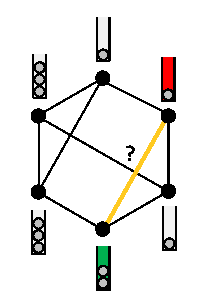
\includegraphics[scale=1.5]{Chapter2/Figs/graphical_two_choice_intro.pdf}
    \caption{One step of the \GraphicalTwoChoice protocol. The decision strategy had to decide between the endpoints of the orange edge, and chose the green one.}
    \label{graphical-two-choice-intro}
\end{figure}

The real-world motivation for this protocol stems from the geographical locality of the servers~\cite{krishnaram2006graphicaltwochoiceoriginal}. One possible implementation of \GraphicalTwoChoice for load balancing is that the client chooses a server $A$ uniformly at random, server $A$ queries the current load of a neighbouring server $B$ chosen uniformly at random, and then $A$ decides whether itself or $B$ should complete the job. In this case the edges correspond to nearby servers, but different underlying graphs are also possible~\cite{peres2015oneplusbeta}, and there are other applications as well, including the efficient storage of hash tables~\cite{krishnaram2006graphicaltwochoiceoriginal}. For this dissertation, I will make the same simplifying assumptions for \GraphicalTwoChoice as discussed for \TwoThinning in Section~\ref{my-approach}.


Note that remarkably, the \Greedy strategy, which allocates the ball into the lesser loaded endpoint of the edge has been shown not to be optimal in general~\cite{bansal2021twochoicegraphical}, therefore this protocol requires a decision strategy, unlike \TwoChoice. I present the first known concrete counterexample for the suboptimality of Greedy in Lemma~\ref{lemma: greedy-suboptimal}.


Analogously, \textsc{Graphical Two-Thinning} is a reasonable protocol too, but I chose to focus on \GraphicalTwoChoice, since there is more literature available on that, so a more thorough comparative evaluation is possible.\\


\subsection{Definitions and Notation} \label{notation}

For the lemmas and conjectures presented in later chapters, it is useful to define and extend some of the above notions formally as well. Let's denote the integers between $0$ and $n-1$ by $[n]$, indicating the indices of the bins.


\begin{definition} [\TwoThinning decision strategy]
A \TwoThinning decision strategy is a function $f$, such that for any load vector $v$ and bin $i\in[n]$, $f(v, i)\in\{\mathrm{accept},\ \mathrm{reject}\}$.
\end{definition}


\begin{definition} [\KThinning decision strategy]
A \KThinning decision strategy is a function $f$, such that for any load vector $v$, bin $i\in[n]$ and $0\leq c<k-1$ indicating the number of bins already rejected for the current ball at $v$, $f(v, i, c)\in\{\mathrm{accept},\ \mathrm{reject}\}$.
\end{definition}


\begin{definition} [slicing strategy]
We call a \TwoThinning (or in general \KThinning) decision strategy \textit{slicing}, if it accepts bin $i$ at load vector $v$ if and only if its load $v[i]$ is less than or equal to a threshold $a$, that can depend on $v$, and for \KThinning also on the number of bins already rejected for the current ball.
\end{definition}


\begin{definition} [threshold function]
Note that a \KThinning \textit{slicing} strategy $f$ can be alternatively defined by a corresponding \textit{threshold function} denoted by $h^f$, such that $h^f(v,c)$ is the threshold used at load $v$ after $c$ rejected bins.
\end{definition}



\begin{definition} [monotone strategy]
We call a \KThinning slicing strategy $f$ \textit{monotone}, if $h^f(v,c)\leq h^f(v,c+1)$ for each $v$ and $0\leq c<k-2$. Intuitively, a monotone strategy never becomes more selective after rejecting a ball.
\end{definition}


\begin{definition} [expected final maximum load]
Let us denote the expected final maximum load of a (decision) strategy $f$ for a protocol $h$ by $E^f_h$, or $E^f$ when $h$ is implicit from the context.
\end{definition}



\subsection{Notes on Related Work and Background Reading}

As part of the preparation, I have read several papers about the theory of balls-into-bins. I present my main findings in Appendix~\ref{related-work}.



\section{Reinforcement Learning} \label{RLintro}


In the Part IB Artificial Intelligence course we have been introduced to supervised learning. While RL is also about optimising an objective function, it differs in several aspects (e.g.\ no labelled data, interactive environment). A very readable introduction to RL can be found in~\cite{sutton2018RLbook}, expanding on my explanation below.


In RL, there is an agent trying to learn an optimal policy by interacting with an environment. It starts in a start state, carries out an action, receives a reward from the environment, observes a new state, and repeats this sequence until it reaches an end state. This process is executed several times (one such run is called an ``episode''), until a sufficiently good policy is learnt. There are several characterisations of RL, but there is a common underlying mathematical model, the so-called Markov Decision Process (MDP) that I will introduce next.

\subsection{Finite Markov Decision Process}


The main component of a Finite MDP is the environment consisting of
\begin{itemize}[itemsep=0pt]
    \item $S$: state space,
    \item $s_0$: start state,
    \item $S_f$: set of final states,
    \item $A(s)$: action space available at state $s$,
    \item $R(s, a, s')$: possible rewards after executing action $a$ in state $s$ and observing next state $s'$, and
    \item $P(s', r \mid s, a)$: the probability of receiving reward $r$ and transitioning to state $s'$ after executing action $a$ in state $s$.
\end{itemize} 


The Markov property has to hold: using timesteps as indices during an execution

\begin{equation} \label{eq:MarkovProperty}
P(s_{t+1},r_{t} \mid s_{t}, a_{t}, s_{t-1}, a_{t-1}, s_{t-2}, a_{t-2}, ..., s_{0}, a_{0}) = P(s_{t+1},r_{t} \mid s_{t}, a_{t})\text{ .}
\end{equation}


The other component of the MDP is an agent that has to learn a \textit{policy}, a function $\pi(a\mid s)$ that assigns probabilities to each of the executable actions in any state. The goal of the agent is to maximise the expected (discounted) cumulative reward collected until the end state:

\begin{equation}\label{eq:cumReward}
\mathbb{E}_{\pi}[r_{0} + \gamma r_{1} + \gamma^2 r_{2} + \gamma^2 r_{3} + \ldots]\text{ ,}
\end{equation}

where $\gamma \in [0, 1]$ is the discount factor, and the sum goes until an end state is reached. Discounting is needed mainly for unbounded MDPs -- where one run can last arbitrarily long -- to avoid divergent rewards. As we will see in Chapter~\ref{implementation}, all our MDPs are bounded -- often even have a fixed number of steps -- so I will set $\gamma=1$ and I will not discuss the more general case from now on.


During training, the agent leans the policy by executing the process several times, i.e.\ starting from the start state, and then interacting with the environment using an carefully chosen policy, until an end state is reached.\\

An example MDP is a simplified version of what I will use for \TwoThinning:

\begin{itemize}[itemsep=0pt]
    \item 
    $S$: load vectors $\{v\in \mathbb{N}^n\mid\mathrm{sum}(v)\triangleq \sum_{i=0}^{n-1}v[i]\leq m\}$,
    \item
    $s_0$: the load configuration no balls,
    \item
    $S_f$: load configurations with $m$ balls,
    \item
    $A(s)$: integer thresholds $0\leq a\leq m$ (meaning that bins with load at most $a$ are the ones accepted),
    \item
    $R(s, a, s')$: the reward is $0$ for $\mathrm{sum}(s')<m$ and $-\mathrm{maxload}(s')\triangleq -\max_{i=0}^{n-1} s[i]$ for $\mathrm{sum}(s')=m$,
    \item
    $P(s', r \mid s, a)$: the probabilities are derived according to the rules of \TwoThinning.
\end{itemize}


\subsection{Fundamentals}

Now I present some standard notions that will be useful for the RL and DP algorithms.


The \textit{state-value function} is the expected cumulative reward of a policy starting from state $s$:

\begin{equation}\label{eq:statevalueFunction}
V_{\pi}(s)=\mathbb{E}_\pi[G_t \mid s_t = s] \text{ ,}
\end{equation}

where the random variable $G_t$ is defined as $r_{t} +  r_{t+1} + r_{t+2} + \ldots$.

For $s=s_0$, we get the expected total cumulative reward of a policy $\pi$, exactly what we aim to maximise. Hence, the optimal policy $\pi^*$ is defined by $\pi^* = \argmax_{\pi} V_{\pi}(s_0)$.


Similarly, the \textit{action-value function} is the expected cumulative reward of a policy starting from state $s$, choosing action $a$:

\begin{equation}\label{eq:actionvalueFunction}
Q_{\pi}(s, a)=\mathbb{E}_\pi[G_t \mid s_t = s, a_t = a] \text{ .}
\end{equation}


The basis of most of the learning algorithms are the Bellman equations~\cite{bellman1957bellmanequation} that characterize the optimal policy recursively:


\begin{equation}\label{eq:bellmanState}
V_{\pi^*}(s) = \max_a \mathbb{E} [r_t + V_{\pi^*}(s_{t+1}) \mid s_t=s, a_t=a]
\end{equation}


\begin{equation} \label{eq:bellmanAction}
Q_{\pi^*}(s,a) = \mathbb{E} [r_t + \max_{a'} Q_{\pi^*}(s_{t+1},a') \mid s_t=s, a_t=a ] 
\end{equation}


Even with these equations, finding the optimal policy is challenging. The two main difficulties are 1) the possible cycles while moving around the state space and 2) the exponentially large size of the state space. As we will see in Chapter~\ref{implementation}, in our cases the state transition graph is acyclic, so the former is not a problem. However, in general, to deal with the latter, the optimal policy has to be approximated.



\subsection{Algorithms}


In all of our protocols, the state space is large (the number of ways $m$ balls can be allocated into $n$ bins is exponentially large), so the agent can focus only on a subset of the states and actions during training. It has to balance between exploring new actions (possibly leading to new states), and gaining confidence in its top actions. This is more generally known as the exploration-exploitation trade-off~\cite{kaelbling1996explorationexploitation}.

The most common approach for dealing with the exploration-exploitation trade-off is the $\epsilon$-greedy technique. During training, the currently best action is chosen with probability $1-\epsilon$ (exploitation) and otherwise the action is chosen uniformly at random (exploration). After training, we set $\epsilon=0$.



\subsubsection*{Q-Learning}


Q-Learning~\cite{watkins1989qlearning} uses the action-value function based Bellman equation~\eqref{eq:bellmanAction}. The algorithm maintains a so-called $Q$-table, such that $Q(s,a)$ stores the current estimates of the action-value function $Q_{\pi^*}(s,a)$ of the optimal policy. The agent executes the process several times using the $\epsilon$-greedy technique based on the current estimates in the $Q$-table. After every step, it updates the $Q$-table using a linear interpolation with smoothing factor $\alpha \in (0,1]$ according to the following update rule:

\begin{equation} \label{eq:q-learningUpdate}
Q(s_t,a_t) \leftarrow Q(s_t,a_t) + \alpha\left( r_t + \max_{a'} Q(s_{t+1}, a')) - Q(s_t,a_t)\right) \text{ .}
\end{equation}


\subsubsection*{\DQL} \label{deepq-learning}


Q-Learning, and its iterative approximation method is a good choice for moderately sized state spaces, where more direct, mainly DP methods are infeasible. However, for exponentially large state spaces, as in our cases, it is infeasible to store the $Q$-table, and also most of its entries would never be updated during training. In \DQL~\cite{mnih2013DQN}, the $Q$-table is approximated using a neural network (NN) $Q_w$ with a tractable number of weights $w$.

Since with function approximations it is not possible to update $Q_w(s, a)$ in isolation, the update rule also has to be adjusted. A natural choice would be to use the gradient of the squared error between the old and the new estimate:

$$\frac{\partial (( r_t + \max_{a'} Q_w(s_{t+1}, a')) - Q_w(s_t,a_t))^2}{\partial w} \text{ .}$$

In practice, due to stability reasons~\cite{barnard1993semigradient}, a semi-gradient is used instead, which essentially treats $Q_{\mathbf{w_t}}(s_{t+1}, a')$ independent of $w$ for the purpose of the differentiation. This yields the final update rule


\begin{equation} \label{eq:deep-q-learning-update-with-semi-gradient}
\mathbf{w} \leftarrow \mathbf{w} + \alpha\left( r_t+ \max_{a'} Q_{\mathbf{w}}(s_{t+1}, a') - Q_{\mathbf{w}}(s_t,a_t)\right)\nabla Q_{\mathbf{w}}(s_{t}, a_t) \text{ .}
\end{equation}

Following standard terminology, I will call the NN used by \DQL as a Deep Q-Network (DQN). I will call the learnt policy as the \DQN strategy.

\subsubsection*{Alternatives}

There are several other algorithms and variants, some of which I implemented and did not outperform \DQL -- see Appendix~\ref{alternativeRL} for further discussion.


\subsection{Recurrent Neural Networks} \label{RNN}


I experimented with several NN architectures for $Q_w$, and here I briefly introduce Recurrent Neural Networks (RNN)~\cite{hopfield1982RNNoriginal}, as they were not covered in the IB Artificial Intelligence or other courses.

RNNs process sequential information by using a hidden state, and updating it by a common weight matrix on every new input (see Figure~\ref{RNN-image}). I used RNNs to obtain an embedding of load vectors, and not to produce an output sequence, as shown in Figure~\ref{RNN-image} for the more general usecase.

\begin{figure}[ht]
    \centering
    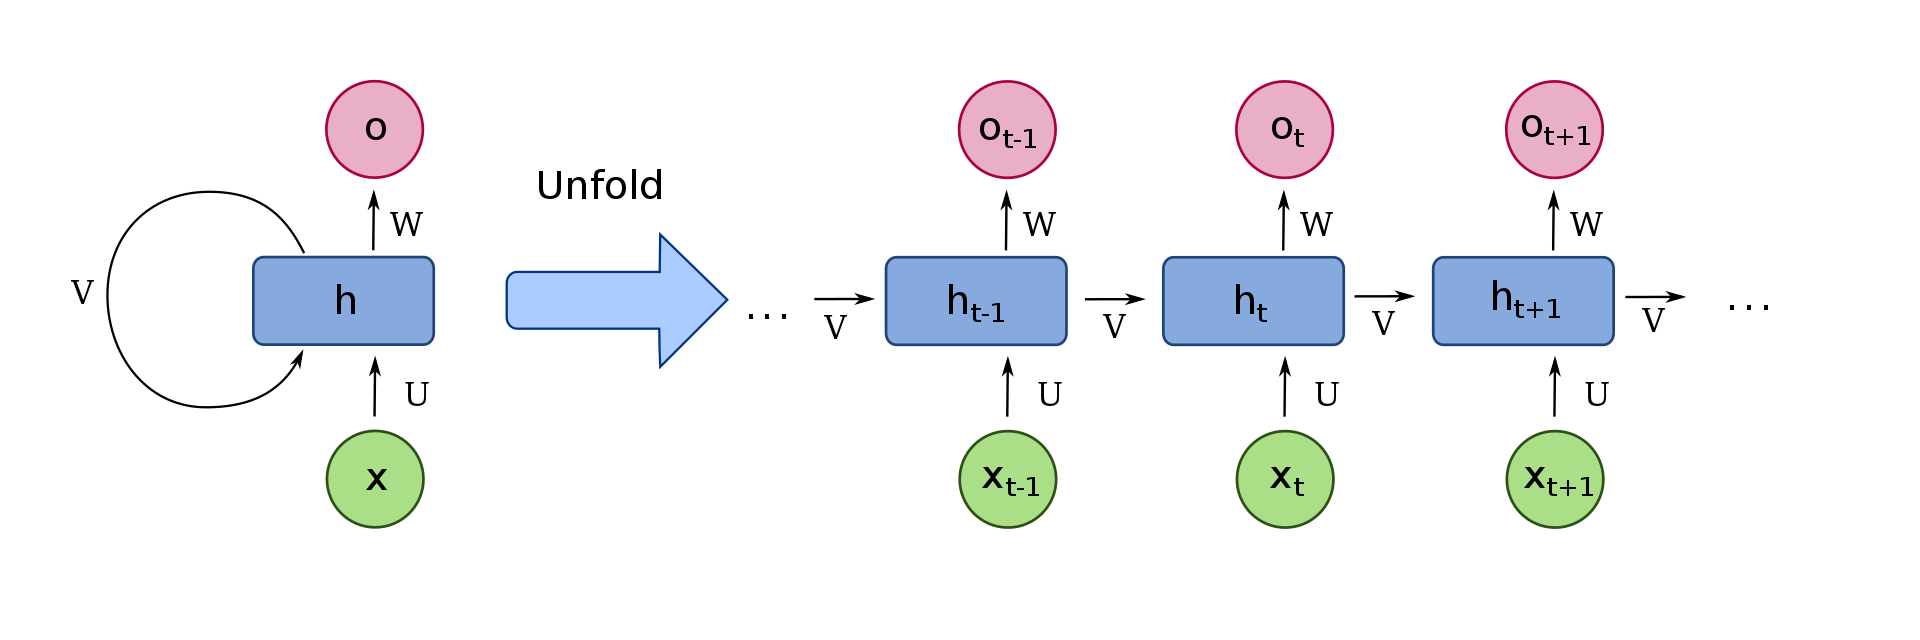
\includegraphics[scale=0.2]{Chapter2/Figs/RNN.png}
    \caption{Two ways of thinking about RNNs~\cite{RNN}.}
     \label{RNN-image}
\end{figure}


\section{Starting Point}

The starting point has not changed since writing the project proposal found in Appendix~\ref{proposal}, no unexpected changes have happened. Before the project, I had no experience in RL and balls-into-bins. I had a solid knowledge of Python and its machine learning libraries, but I had never used them for RL. The project does not rely on any existing codebase, apart from common open-source Python libraries, as discussed in Section~\ref{software-and-hardware}.


\section{Requirements Analysis and Risk Assessment}

In this section I present the requirements of the projects, the corresponding estimated risks before the start, and some reflections after completing the requirements.

\begin{itemize}

    \item \textbf{Background Reading}: \textcolor{YellowOrange}{medium risk}, \textcolor{Red}{high difficulty}
    
    I had no previous knowledge about RL or balls-into-bins beyond related foundational courses from the Tripos, so I have done extensive background reading in both, gaining a deep understanding of the balls-into-bins literature, and exploring the relevant parts of RL.
    
    The biggest challenge was understanding the proofs in balls-into-bins papers, which I considered an extension. I eventually succeeded and gained valuable insights.
    
    \item \textbf{Implementing Deep Reinforcement Learning}: \textcolor{red}{high risk}, \textcolor{red}{high difficulty}
    
    The main risk involved in this main component was the uncertainty whether RL, being a novel approach to balls-into-bins, will actually perform well in learning decision strategies.
    
    The main difficulty was optimising \DQL for better results (see Section~\ref{improvementideas}).
    
    \item \textbf{Implementing Other Strategies}: \textcolor{green}{low risk}, \textcolor{YellowOrange}{medium difficulty}
    Having done much competitive programming, I was confident in my algorithmic knowledge, so I could efficiently develop and implement algorithms, such as dynamic programming.
    
    \item \textbf{Evaluation}: \textcolor{YellowOrange}{medium risk}, \textcolor{YellowOrange}{medium difficulty}
    
    The medium risk stemmed from the novelty of my non-asymptotic approach, and the time it took to compare the strategies with acceptable confidence intervals.
    
    The hardest part about evaluation was finding the most insightful analyses for explaining the behaviour of strategies.
    
\end{itemize}


\section{Software Engineering Methodology}


\subsection{Software and Hardware} \label{software-and-hardware}


For this project I used Python, due to its flexibility for quick experimentation, its extensive library support with strong community (e.g.\ numpy~\cite{harris2020numpy} for vectorised computation, Pytorch~\cite{paszke2019pytorch} for deep learning), and its object oriented features. As there is no prior work on RL for the discussed balls-into-bins protocols, I implemented the RL algorithms from scratch using PyTorch for the NNs. Even though there are some attempts at general purpose RL libraries, such as Stable Baselines~\cite{hill2018stablebaselines}, they are very hard to customise at the moment. I used the PyCharm IDE for its powerful debugger and its ability to seamlessly parallelise tasks.


I used my laptop for all experiments and its details are: \texttt{Intel(R) Core(TM) i7-8565U CPU @ 1.80GHz, 1992 Mhz, 4 Cores, 8 Logical Processors, NVIDIA GeForce MX150 GPU}. Gaining the expected speedup from GPUs for RL is not an easy problem, due to the difficulty of batching for a MDP~\cite{stooke2018gpudeepRL} (see Section~\ref{evaluationnotes} for my approach).


\subsection{Project Management}

I used Git for version control and Google Drive as a secondary backup, taking monthly copies. I used the work plan in my project proposal as the target schedule, interleaving evaluation and implementation work to gain better insights about what to focus on. Due to the large number of components in the RL algorithms (see Sections~\ref{dqn-implmentation-two-thinning} and~\ref{improvementideas}), I applied an iterative approach to the implementation, making sure each new component added has the desired effect. We had biweekly meetings with my supervisors, where we came up with several ideas and analysed my results from the perspective of the closely related research they are doing. I maintained a logbook that later served as the baseline for my dissertation.